\chapter{Mexican Axolotl Optimization}

Los dioses mexicas se reunieron en Teotihuacan para crear el universo ofreciendo su propia vida en sacrificio. Dioses como Huitzilopochtli, Xochipilli y Tezcatlipoca tomaron el sacrificio, sin embargo, Xolotl, victima del miedo, huyo del ritual. 

Xolotl se transformo en múltiples criaturas para evitar se atrapado por el viento, se transformo en diferentes criaturas pero seguía siendo encontrado, por lo que opto por arrojarse al lago convirtiéndose en un anfibio con branquias en forma de cuernos, un axolote. Pudo sobrevivir algunos días en el lago pero finalmente fue atrapado por el viento y llevado al ritual para dar movimiento al universo \cite{leyenda}.

\section{Modelo natural}

El axolote mexicano o \textit{Ambystoma mexicanum} es una especie endémica del lago de Xochimilco, son salamandras que nunca superan su fase larvaria. Tiene branquias que brotan de su cabeza, patas palmeadas, una aleta dorsal, cola, pulmones funcionales, camuflaje y una sonrisa.

Los axolotes son un tema de investigación por biólogos dado a su capacidad de regenerar extremidades y órganos sin cicatrices permanentes \cite{axolote}.

\section{Modelo artificial}

 El algoritmo \textit{Mexican Axolotl Optimization} (\textbf{MAO}) busca imitar el comportamiento de estos anfibios para encontrar la mejor solución en un espacio de búsqueda dadas las siguientes analogías:
 
 \begin{itemize}
 	\item Los ajolotes son soluciones de problemas y sus órganos y extremidades las dimensiones de la solución.
 	\item El lago en donde viven es el espacio de búsqueda.
 	\item El camuflaje del axolote, cuya efectividad depende del estado de búsqueda, determina la capacidad de sobrevivir, es decir, su aptitud.
 \end{itemize}
 
 En otras palabras, sea $O$ un problema de optmización numerica cuyas elementos sea vectores de dimensión $D$ acotados en el rango $[\min_i, \max_i]$, los axolotes representan un conjunto de soluciones de tamaño $np$: $P = \{ S_1, \dots, S_{np} \}$ donde $O(S_j) \in \mathbb{R} \; \forall j \in \{1, \dots,  np\}$.
 
 El algoritmo MAO es un proceso iterativo de 4 etapas definida por el acronimo \textit{TIRA}: transición de larva a adulto (\textit{Transition}), lesión y restauración \textit{Injury and restoration}, reproducción (\textit{Reproduction}) y variedad (\textit{Assortment}).
 
 \subsection{Transition}
 
 La población de axolotes se inicia de manera aleatoria y a cada individuo se le asigna un genero, obteniendo dos subconjuntos. Los individuos de cada grupo transicionan en el agua de larvas a adultos ajustando el color de las partes de su cuerpo para parecerse mas al mejor de cada grupo, como se muestra en el algoritmo \ref{alg:transition}
 
 \begin{algorithm}
 	\caption{Transition \\
 	\textbf{Input} constante de diferenciación $\alpha$, Población $P$, Función de optimización $O$ \\
 	\textbf{Output}  Población actualizada $P'$} 
 	\begin{algorithmic}[1]
 		\State El mejor axolote: $p_{best} = Best(P)$
 		\For{$p_j \in P $}
 			\State Probabilidad inversa de transición: $pp_j = \frac{O(p_j)}{\sum O(p_i)}$
 			\If{$pp_j < r$}
 				\State Se aproxima al mejor: $p_{j,i} = p_{j,i} + (p_{best, i} - p_{j,i}) \cdot \alpha $
 			\Else
 				\State Se mueve de forma aleatoria: $p_{j,i} = \min_i + (\max_i - \min_i) * r_i$
 			\EndIf
 		\EndFor 
 	\end{algorithmic}
 	\label{alg:transition}
 \end{algorithm}
 
 La habilidad de los ajolotes de cambiar de color esta limitada, por lo que unicamente se aproximan a la nueva solución, ya que no se busca que se adapten de forma perfecta al mejor de ellos. Cuando los individuos son difieren mucho de la mejor solución, medida que se obtiene con la probabilidad inversa, se mueven de manera aleatoria para explorar el espacio.
 
 \subsection{Injury and restoration}
 
 Mientras los axolotes se mueven en el agua pueden sufrir accidentes y ser lastimados. En esta fase los ajolotes pierden partes que posteriormente regeneran de forma aleatoria, para esto, se consideran ambas probabilidades donde la primera actuá sobre los axolotes que serán lastimados y la segunda sobre las partes del cuerpo que serán regeneradas, esto se aplica para ambos grupos como se muestra en el algoritmo \ref{alg:injury}.
 
  \begin{algorithm}
 	\caption{Injury and Restoration \\
 		\textbf{Input} Población $P$, probabilidad de daño $dp$, probabilidad de regeneración $rp$ \\
 		\textbf{Output}  Población actualizada $P'$} 
 	\begin{algorithmic}[1]
 		\For{ $p_j \in P$}
 			\If{$r \leq dp$}
 				\For{$i \in D$}
 					\If{$r \leq rp$}
 						\State $p_{j,i} = \min_i + (\max_i - \min_i) * r_i$
 					\EndIf
 				\EndFor
 			\EndIf
 		\EndFor
 	\end{algorithmic}
 	\label{alg:injury}
 \end{algorithm}
 
 \subsection{Reproduction and Assortment}
 
 Los machos y las hembras se reproducen dejando un par de huevos que contienen una mezcla del material genético de los padres de forma uniforme. Se genera una cadena aleatoria de tamaño $D$ y si es un 0 el primer hijo hereda el gen del padre y el dos de la madre, si es un 1 el primer hijo hereda del gen de la madre y el dos del padre, como se muestra en la figura \ref{fig:uniform}.

 \begin{figure}[H]
 	\centering
 	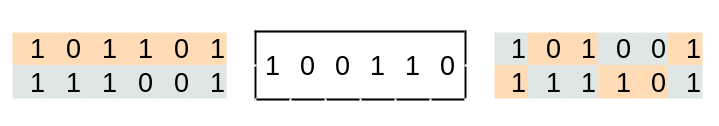
\includegraphics[width=0.75\linewidth]{img/cross_uniform.png}
 	\caption{Cruza uniforme}
 	\label{fig:uniform}
 \end{figure}
 
 El algoritmo \ref{alg:resproduction} selecciona, entre un rango de machos, con quien reproducirse mediante un torneo de tamaño $k$ con cada hembra, cuyos huevos heredan el material genético. Finalmente, entre los 4 individuos se seleccionan los dos mejores y se les asigna el genero de hembra y macho al primero y segundo mejor respectivamente.
 
   \begin{algorithm}[H]
 	\caption{Reproduction \\
 		\textbf{Input} Población $P$, probabilidad de daño $dp$, probabilidad de regeneración $rp$ \\
 		\textbf{Output}  Población actualizada $P'$} 
 	\begin{algorithmic}[1]
 		\For{ $f \in F$}
 			\State $m = \{Best(MC) | MC \subset M \land |MC| = k\}$
 			\State egg$_1$
 			\State egg$_2$
 			\For{$i \in D$}
 				\If{$r \leq 0.5$}
 					\State huevo$_{1,i} = m_i$
 					\State huevo$_{2,i} = f_i$ 
 				\Else
 					\State huevo$_{1,i} = f_i$
 					\State huevo$_{2,i} = m_i$ 
 				\EndIf
 			\EndFor
 		\EndFor
 		\State $V=Sort(function= O, \{ f, m, \text{huevo}_1, \text{huevo}_2 \})$
 		\State $f = V[0]$
 		\State $m = V[1]$
 	\end{algorithmic}
 	\label{alg:resproduction}
 \end{algorithm}
 


 
 